\begin{frame}{Problems that Longest Path Problem Reduces To}
    We now take a look at problems that can be reduced from longest path problem.
    \begin{itemize}
        \item <2-> Travelling Salesman Problem
        \item[] <3-> \begin{block}{\textbf{Result}}
                {Longest Path Problem $\leq_p$ Travelling Salesman Problem}
            \end{block}
        \item <4-> Two formulation of the Travelling Salesman Problem can be considered. In one version, the salesman visits each city(vertices) once and the other is more general where each city(vertices) may be visited more than once.
        \item <5-> Both of these cases can be reduced to finding the longest path between two nodes in a finite, connected graph.
        
    \end{itemize}
\end{frame}

\begin{frame}{Problems that Longest Path Problem Reduces To}
    

\tikzset{every picture/.style={line width=0.70pt}} %set default line width to 0.75pt        

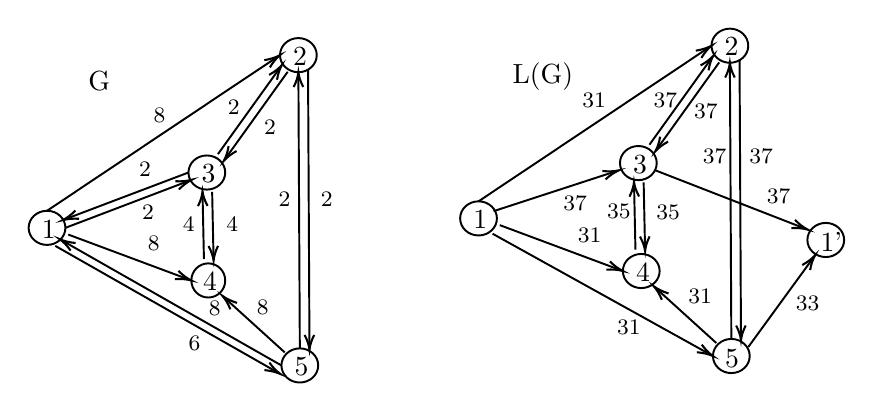
\begin{tikzpicture}[x=0.75pt,y=0.75pt,yscale=-0.65,xscale=0.70]
%uncomment if require: \path (0,442); %set diagram left start at 0, and has height of 442

%Shape: Circle [id:dp6082651193246167] 
\draw   (210,54.85) .. controls (210,47.86) and (215.66,42.2) .. (222.65,42.2) .. controls (229.64,42.2) and (235.3,47.86) .. (235.3,54.85) .. controls (235.3,61.84) and (229.64,67.5) .. (222.65,67.5) .. controls (215.66,67.5) and (210,61.84) .. (210,54.85) -- cycle ;

%Straight Lines [id:da4796217542898069] 
\draw    (229.3,65.2) -- (230.29,271.2) ;
\draw [shift={(230.3,273.2)}, rotate = 269.72] [color={rgb, 255:red, 0; green, 0; blue, 0 }  ][line width=0.75]    (10.93,-3.29) .. controls (6.95,-1.4) and (3.31,-0.3) .. (0,0) .. controls (3.31,0.3) and (6.95,1.4) .. (10.93,3.29)   ;
%Straight Lines [id:da7462639427922131] 
\draw    (222.66,69.5) -- (223.65,272.2) ;
\draw [shift={(222.65,67.5)}, rotate = 89.72] [color={rgb, 255:red, 0; green, 0; blue, 0 }  ][line width=0.75]    (10.93,-3.29) .. controls (6.95,-1.4) and (3.31,-0.3) .. (0,0) .. controls (3.31,0.3) and (6.95,1.4) .. (10.93,3.29)   ;
%Shape: Circle [id:dp6767693430221662] 
\draw   (211,284.85) .. controls (211,277.86) and (216.66,272.2) .. (223.65,272.2) .. controls (230.64,272.2) and (236.3,277.86) .. (236.3,284.85) .. controls (236.3,291.84) and (230.64,297.5) .. (223.65,297.5) .. controls (216.66,297.5) and (211,291.84) .. (211,284.85) -- cycle ;

%Shape: Ellipse [id:dp9047480014872011] 
\draw   (149,221.85) .. controls (149,214.86) and (154.22,209.2) .. (160.65,209.2) .. controls (167.08,209.2) and (172.3,214.86) .. (172.3,221.85) .. controls (172.3,228.84) and (167.08,234.5) .. (160.65,234.5) .. controls (154.22,234.5) and (149,228.84) .. (149,221.85) -- cycle ;

%Shape: Circle [id:dp7029760309478779] 
\draw   (147,141.85) .. controls (147,134.86) and (152.66,129.2) .. (159.65,129.2) .. controls (166.64,129.2) and (172.3,134.86) .. (172.3,141.85) .. controls (172.3,148.84) and (166.64,154.5) .. (159.65,154.5) .. controls (152.66,154.5) and (147,148.84) .. (147,141.85) -- cycle ;

%Shape: Circle [id:dp3710280826915211] 
\draw   (37,182.85) .. controls (37,175.86) and (42.66,170.2) .. (49.65,170.2) .. controls (56.64,170.2) and (62.3,175.86) .. (62.3,182.85) .. controls (62.3,189.84) and (56.64,195.5) .. (49.65,195.5) .. controls (42.66,195.5) and (37,189.84) .. (37,182.85) -- cycle ;

%Straight Lines [id:da29462268616093246] 
\draw    (215.3,67.2) -- (172.41,131.54) ;
\draw [shift={(171.3,133.2)}, rotate = 303.69] [color={rgb, 255:red, 0; green, 0; blue, 0 }  ][line width=0.75]    (10.93,-3.29) .. controls (6.95,-1.4) and (3.31,-0.3) .. (0,0) .. controls (3.31,0.3) and (6.95,1.4) .. (10.93,3.29)   ;
%Straight Lines [id:da6028840278191208] 
\draw    (210.19,63.86) -- (167.3,128.2) ;
\draw [shift={(211.3,62.2)}, rotate = 123.69] [color={rgb, 255:red, 0; green, 0; blue, 0 }  ][line width=0.75]    (10.93,-3.29) .. controls (6.95,-1.4) and (3.31,-0.3) .. (0,0) .. controls (3.31,0.3) and (6.95,1.4) .. (10.93,3.29)   ;
%Straight Lines [id:da06383174973927552] 
\draw    (163.3,156.2) -- (164.26,205.2) ;
\draw [shift={(164.3,207.2)}, rotate = 268.88] [color={rgb, 255:red, 0; green, 0; blue, 0 }  ][line width=0.75]    (10.93,-3.29) .. controls (6.95,-1.4) and (3.31,-0.3) .. (0,0) .. controls (3.31,0.3) and (6.95,1.4) .. (10.93,3.29)   ;
%Straight Lines [id:da4218809481340329] 
\draw    (156.69,157.76) -- (157.65,205.95) ;
\draw [shift={(156.65,155.76)}, rotate = 88.86] [color={rgb, 255:red, 0; green, 0; blue, 0 }  ][line width=0.75]    (10.93,-3.29) .. controls (6.95,-1.4) and (3.31,-0.3) .. (0,0) .. controls (3.31,0.3) and (6.95,1.4) .. (10.93,3.29)   ;
%Straight Lines [id:da2468655944407605] 
\draw    (171.73,234.6) -- (213.3,275.2) ;
\draw [shift={(170.3,233.2)}, rotate = 44.33] [color={rgb, 255:red, 0; green, 0; blue, 0 }  ][line width=0.75]    (10.93,-3.29) .. controls (6.95,-1.4) and (3.31,-0.3) .. (0,0) .. controls (3.31,0.3) and (6.95,1.4) .. (10.93,3.29)   ;
%Straight Lines [id:da8916503878094448] 
\draw    (55.3,196.2) -- (208.59,290.15) ;
\draw [shift={(210.3,291.2)}, rotate = 211.5] [color={rgb, 255:red, 0; green, 0; blue, 0 }  ][line width=0.75]    (10.93,-3.29) .. controls (6.95,-1.4) and (3.31,-0.3) .. (0,0) .. controls (3.31,0.3) and (6.95,1.4) .. (10.93,3.29)   ;
%Straight Lines [id:da7392607272022387] 
\draw    (60,192.25) -- (211,284.85) ;
\draw [shift={(58.3,191.2)}, rotate = 31.52] [color={rgb, 255:red, 0; green, 0; blue, 0 }  ][line width=0.75]    (10.93,-3.29) .. controls (6.95,-1.4) and (3.31,-0.3) .. (0,0) .. controls (3.31,0.3) and (6.95,1.4) .. (10.93,3.29)   ;
%Straight Lines [id:da22957493465129608] 
\draw    (62.3,182.85) -- (147.45,147.96) ;
\draw [shift={(149.3,147.2)}, rotate = 517.72] [color={rgb, 255:red, 0; green, 0; blue, 0 }  ][line width=0.75]    (10.93,-3.29) .. controls (6.95,-1.4) and (3.31,-0.3) .. (0,0) .. controls (3.31,0.3) and (6.95,1.4) .. (10.93,3.29)   ;
%Straight Lines [id:da8649335227093395] 
\draw    (62.15,176.44) -- (147,141.85) ;
\draw [shift={(60.3,177.2)}, rotate = 337.82] [color={rgb, 255:red, 0; green, 0; blue, 0 }  ][line width=0.75]    (10.93,-3.29) .. controls (6.95,-1.4) and (3.31,-0.3) .. (0,0) .. controls (3.31,0.3) and (6.95,1.4) .. (10.93,3.29)   ;
%Straight Lines [id:da05809272007118116] 
\draw    (64.3,187.85) -- (147.14,221.1) ;
\draw [shift={(149,221.85)}, rotate = 201.87] [color={rgb, 255:red, 0; green, 0; blue, 0 }  ][line width=0.75]    (10.93,-3.29) .. controls (6.95,-1.4) and (3.31,-0.3) .. (0,0) .. controls (3.31,0.3) and (6.95,1.4) .. (10.93,3.29)   ;
%Straight Lines [id:da44302434198929097] 
\draw    (49.65,170.2) -- (208.38,56.02) ;
\draw [shift={(210,54.85)}, rotate = 504.27] [color={rgb, 255:red, 0; green, 0; blue, 0 }  ][line width=0.75]    (10.93,-3.29) .. controls (6.95,-1.4) and (3.31,-0.3) .. (0,0) .. controls (3.31,0.3) and (6.95,1.4) .. (10.93,3.29)   ;
%Shape: Circle [id:dp12337037116319083] 
\draw   (507,47.85) .. controls (507,40.86) and (512.66,35.2) .. (519.65,35.2) .. controls (526.64,35.2) and (532.3,40.86) .. (532.3,47.85) .. controls (532.3,54.84) and (526.64,60.5) .. (519.65,60.5) .. controls (512.66,60.5) and (507,54.84) .. (507,47.85) -- cycle ;

%Straight Lines [id:da6971974699136669] 
\draw    (526.3,58.2) -- (527.29,264.2) ;
\draw [shift={(527.3,266.2)}, rotate = 269.72] [color={rgb, 255:red, 0; green, 0; blue, 0 }  ][line width=0.75]    (10.93,-3.29) .. controls (6.95,-1.4) and (3.31,-0.3) .. (0,0) .. controls (3.31,0.3) and (6.95,1.4) .. (10.93,3.29)   ;
%Straight Lines [id:da6162591979171923] 
\draw    (519.66,62.5) -- (520.65,265.2) ;
\draw [shift={(519.65,60.5)}, rotate = 89.72] [color={rgb, 255:red, 0; green, 0; blue, 0 }  ][line width=0.75]    (10.93,-3.29) .. controls (6.95,-1.4) and (3.31,-0.3) .. (0,0) .. controls (3.31,0.3) and (6.95,1.4) .. (10.93,3.29)   ;
%Shape: Circle [id:dp45403978795594546] 
\draw   (508,277.85) .. controls (508,270.86) and (513.66,265.2) .. (520.65,265.2) .. controls (527.64,265.2) and (533.3,270.86) .. (533.3,277.85) .. controls (533.3,284.84) and (527.64,290.5) .. (520.65,290.5) .. controls (513.66,290.5) and (508,284.84) .. (508,277.85) -- cycle ;

%Shape: Circle [id:dp6556703904433001] 
\draw   (446,214.85) .. controls (446,207.86) and (451.66,202.2) .. (458.65,202.2) .. controls (465.64,202.2) and (471.3,207.86) .. (471.3,214.85) .. controls (471.3,221.84) and (465.64,227.5) .. (458.65,227.5) .. controls (451.66,227.5) and (446,221.84) .. (446,214.85) -- cycle ;

%Shape: Circle [id:dp11649025123762113] 
\draw   (444,134.85) .. controls (444,127.86) and (449.66,122.2) .. (456.65,122.2) .. controls (463.64,122.2) and (469.3,127.86) .. (469.3,134.85) .. controls (469.3,141.84) and (463.64,147.5) .. (456.65,147.5) .. controls (449.66,147.5) and (444,141.84) .. (444,134.85) -- cycle ;

%Shape: Circle [id:dp902034539249932] 
\draw   (334,175.85) .. controls (334,168.86) and (339.66,163.2) .. (346.65,163.2) .. controls (353.64,163.2) and (359.3,168.86) .. (359.3,175.85) .. controls (359.3,182.84) and (353.64,188.5) .. (346.65,188.5) .. controls (339.66,188.5) and (334,182.84) .. (334,175.85) -- cycle ;

%Straight Lines [id:da027918768168032848] 
\draw    (512.3,60.2) -- (469.41,124.54) ;
\draw [shift={(468.3,126.2)}, rotate = 303.69] [color={rgb, 255:red, 0; green, 0; blue, 0 }  ][line width=0.75]    (10.93,-3.29) .. controls (6.95,-1.4) and (3.31,-0.3) .. (0,0) .. controls (3.31,0.3) and (6.95,1.4) .. (10.93,3.29)   ;
%Straight Lines [id:da307052577675168] 
\draw    (507.19,56.86) -- (464.3,121.2) ;
\draw [shift={(508.3,55.2)}, rotate = 123.69] [color={rgb, 255:red, 0; green, 0; blue, 0 }  ][line width=0.75]    (10.93,-3.29) .. controls (6.95,-1.4) and (3.31,-0.3) .. (0,0) .. controls (3.31,0.3) and (6.95,1.4) .. (10.93,3.29)   ;
%Straight Lines [id:da3503065238284948] 
\draw    (460.3,149.2) -- (461.26,198.2) ;
\draw [shift={(461.3,200.2)}, rotate = 268.88] [color={rgb, 255:red, 0; green, 0; blue, 0 }  ][line width=0.75]    (10.93,-3.29) .. controls (6.95,-1.4) and (3.31,-0.3) .. (0,0) .. controls (3.31,0.3) and (6.95,1.4) .. (10.93,3.29)   ;
%Straight Lines [id:da4090177414512237] 
\draw    (453.69,150.76) -- (454.65,198.95) ;
\draw [shift={(453.65,148.76)}, rotate = 88.86] [color={rgb, 255:red, 0; green, 0; blue, 0 }  ][line width=0.75]    (10.93,-3.29) .. controls (6.95,-1.4) and (3.31,-0.3) .. (0,0) .. controls (3.31,0.3) and (6.95,1.4) .. (10.93,3.29)   ;
%Straight Lines [id:da9976508386876173] 
\draw    (468.73,227.6) -- (510.3,268.2) ;
\draw [shift={(467.3,226.2)}, rotate = 44.33] [color={rgb, 255:red, 0; green, 0; blue, 0 }  ][line width=0.75]    (10.93,-3.29) .. controls (6.95,-1.4) and (3.31,-0.3) .. (0,0) .. controls (3.31,0.3) and (6.95,1.4) .. (10.93,3.29)   ;
%Straight Lines [id:da20695360152203035] 
\draw    (356.3,187.2) -- (506.28,276.82) ;
\draw [shift={(508,277.85)}, rotate = 210.86] [color={rgb, 255:red, 0; green, 0; blue, 0 }  ][line width=0.75]    (10.93,-3.29) .. controls (6.95,-1.4) and (3.31,-0.3) .. (0,0) .. controls (3.31,0.3) and (6.95,1.4) .. (10.93,3.29)   ;
%Straight Lines [id:da8563754699020032] 
\draw    (357,170.5) -- (441.41,140.86) ;
\draw [shift={(443.3,140.2)}, rotate = 520.65] [color={rgb, 255:red, 0; green, 0; blue, 0 }  ][line width=0.75]    (10.93,-3.29) .. controls (6.95,-1.4) and (3.31,-0.3) .. (0,0) .. controls (3.31,0.3) and (6.95,1.4) .. (10.93,3.29)   ;
%Straight Lines [id:da5535602138752693] 
\draw    (361.3,180.85) -- (444.14,214.1) ;
\draw [shift={(446,214.85)}, rotate = 201.87] [color={rgb, 255:red, 0; green, 0; blue, 0 }  ][line width=0.75]    (10.93,-3.29) .. controls (6.95,-1.4) and (3.31,-0.3) .. (0,0) .. controls (3.31,0.3) and (6.95,1.4) .. (10.93,3.29)   ;
%Straight Lines [id:da08156888775185767] 
\draw    (346.65,163.2) -- (505.38,49.02) ;
\draw [shift={(507,47.85)}, rotate = 504.27] [color={rgb, 255:red, 0; green, 0; blue, 0 }  ][line width=0.75]    (10.93,-3.29) .. controls (6.95,-1.4) and (3.31,-0.3) .. (0,0) .. controls (3.31,0.3) and (6.95,1.4) .. (10.93,3.29)   ;
%Shape: Circle [id:dp41985773772062474] 
\draw   (573,191.85) .. controls (573,184.86) and (578.66,179.2) .. (585.65,179.2) .. controls (592.64,179.2) and (598.3,184.86) .. (598.3,191.85) .. controls (598.3,198.84) and (592.64,204.5) .. (585.65,204.5) .. controls (578.66,204.5) and (573,198.84) .. (573,191.85) -- cycle ;

%Straight Lines [id:da5769895810285448] 
\draw    (468.3,140.2) -- (571.46,183.43) ;
\draw [shift={(573.3,184.2)}, rotate = 202.74] [color={rgb, 255:red, 0; green, 0; blue, 0 }  ][line width=0.75]    (10.93,-3.29) .. controls (6.95,-1.4) and (3.31,-0.3) .. (0,0) .. controls (3.31,0.3) and (6.95,1.4) .. (10.93,3.29)   ;
%Straight Lines [id:da38975406545115066] 
\draw    (532.3,271.2) -- (577.18,204.86) ;
\draw [shift={(578.3,203.2)}, rotate = 484.08] [color={rgb, 255:red, 0; green, 0; blue, 0 }  ][line width=0.75]    (10.93,-3.29) .. controls (6.95,-1.4) and (3.31,-0.3) .. (0,0) .. controls (3.31,0.3) and (6.95,1.4) .. (10.93,3.29)   ;

% Text Node
\draw (236,154) node [anchor=north west][inner sep=0.75pt]   [align=left] {{\footnotesize 2}};
% Text Node
\draw (207,154) node [anchor=north west][inner sep=0.75pt]   [align=left] {{\footnotesize 2}};
% Text Node
\draw (197,101) node [anchor=north west][inner sep=0.75pt]   [align=left] {{\footnotesize 2}};
% Text Node
\draw (172,86) node [anchor=north west][inner sep=0.75pt]   [align=left] {{\footnotesize 2}};
% Text Node
\draw (113,164) node [anchor=north west][inner sep=0.75pt]   [align=left] {{\footnotesize 2}};
% Text Node
\draw (111,132) node [anchor=north west][inner sep=0.75pt]   [align=left] {{\footnotesize 2}};
% Text Node
\draw (171,173) node [anchor=north west][inner sep=0.75pt]   [align=left] {{\footnotesize 4}};
% Text Node
\draw (141,173) node [anchor=north west][inner sep=0.75pt]   [align=left] {{\footnotesize 4}};
% Text Node
\draw (117,187) node [anchor=north west][inner sep=0.75pt]   [align=left] {{\footnotesize 8}};
% Text Node
\draw (192,234) node [anchor=north west][inner sep=0.75pt]   [align=left] {{\footnotesize 8}};
% Text Node
\draw (145,261) node [anchor=north west][inner sep=0.75pt]   [align=left] {{\footnotesize 6}};
% Text Node
\draw (159,235) node [anchor=north west][inner sep=0.75pt]   [align=left] {{\footnotesize 8}};
% Text Node
\draw (121,92) node [anchor=north west][inner sep=0.75pt]   [align=left] {{\footnotesize 8}};
% Text Node
\draw (76,65) node [anchor=north west][inner sep=0.75pt]   [align=left] {G};
% Text Node
\draw (531,122) node [anchor=north west][inner sep=0.75pt]   [align=left] {{\footnotesize 37}};
% Text Node
\draw (499,122) node [anchor=north west][inner sep=0.75pt]   [align=left] {{\footnotesize 37}};
% Text Node
\draw (493,89) node [anchor=north west][inner sep=0.75pt]   [align=left] {{\footnotesize 37}};
% Text Node
\draw (465,81) node [anchor=north west][inner sep=0.75pt]   [align=left] {{\footnotesize 37}};
% Text Node
\draw (403,157) node [anchor=north west][inner sep=0.75pt]   [align=left] {{\footnotesize 37}};
% Text Node
\draw (467,164) node [anchor=north west][inner sep=0.75pt]   [align=left] {{\footnotesize 35}};
% Text Node
\draw (433,163) node [anchor=north west][inner sep=0.75pt]   [align=left] {{\footnotesize 35}};
% Text Node
\draw (413,181) node [anchor=north west][inner sep=0.75pt]   [align=left] {{\footnotesize 31}};
% Text Node
\draw (489,226) node [anchor=north west][inner sep=0.75pt]   [align=left] {{\footnotesize 31}};
% Text Node
\draw (440,249) node [anchor=north west][inner sep=0.75pt]   [align=left] {{\footnotesize 31}};
% Text Node
\draw (416,81) node [anchor=north west][inner sep=0.75pt]   [align=left] {{\footnotesize 31}};
% Text Node
\draw (368,58) node [anchor=north west][inner sep=0.75pt]   [align=left] {L(G)};
% Text Node
\draw (543,152) node [anchor=north west][inner sep=0.75pt]   [align=left] {{\footnotesize 37}};
% Text Node
\draw (563,231) node [anchor=north west][inner sep=0.75pt]   [align=left] {{\footnotesize 33}};
% Text Node
\draw (44,175) node [anchor=north west][inner sep=0.75pt]   [align=left] {1};
% Text Node
\draw (154,134) node [anchor=north west][inner sep=0.75pt]   [align=left] {3};
% Text Node
\draw (217,47) node [anchor=north west][inner sep=0.75pt]   [align=left] {2};
% Text Node
\draw (155.01,214) node [anchor=north west][inner sep=0.75pt]   [align=left] {4};
% Text Node
\draw (218,277) node [anchor=north west][inner sep=0.75pt]   [align=left] {5};
% Text Node
\draw (341,168) node [anchor=north west][inner sep=0.75pt]   [align=left] {1};
% Text Node
\draw (451,127) node [anchor=north west][inner sep=0.75pt]   [align=left] {3};
% Text Node
\draw (514,40) node [anchor=north west][inner sep=0.75pt]   [align=left] {2};
% Text Node
\draw (453,207) node [anchor=north west][inner sep=0.75pt]   [align=left] {4};
% Text Node
\draw (514.3,271.2) node [anchor=north west][inner sep=0.75pt]   [align=left] {5};
% Text Node
\draw (580,184) node [anchor=north west][inner sep=0.75pt]   [align=left] {1'};


\end{tikzpicture}
    \begin{itemize}
        \item <1-> The construction of \textit{L(G)} from \textit{G}, with $S=8+8+8+8+6 = 38$ and $K$ taken to be $39$; the optimal cycle in $G$ is $(1,4,3,2,5)$ and the longest path in $L(G)$ is $(1,4,3,2,5,1')$.
        \item <2->However, we couldn't find any other problem that longest path problem naturally reduces to.
        
    \end{itemize}
\end{frame}

% \begin{frame}{Problems that Longest Path Problem Reduces To}
%     \begin{itemize}
%         \item <1-> The construction of \textit{L(G)} from \textit{G}, with $S=8+8+8+8+6 = 38$ and $K$ taken to be $39$; the optimal cycle in $G$ is $(1,4,3,2,5)$ and the longest path in $L(G)$ is $(1,4,3,2,5,1')$.
        
%         \item <2->$K$ must be strictly greater than $S$. Otherwise, the reduction will not satisfy.
        
%         \item <3->However, we couldn't find any other problem that longest path problem naturally reduces to.
%     \end{itemize}
% \end{frame}
